\documentclass[aspectratio=169,11pt]{beamer}
\usetheme{Madrid}
\usecolortheme{seahorse}
\usepackage[utf8]{inputenc}
\usepackage[T1]{fontenc}
\usepackage{lmodern}
\usepackage{amsmath,amssymb}
\usepackage{graphicx}
\usepackage{booktabs}
\usepackage{array}
\usepackage{tikz}
\usetikzlibrary{arrows.meta,positioning}

\setbeamertemplate{navigation symbols}{}
\definecolor{iteraBlue}{RGB}{23,70,125}
\definecolor{iteraGold}{RGB}{175,145,55}
\definecolor{softBlue}{RGB}{235,242,250}
\setbeamercolor{title}{fg=iteraBlue}
\setbeamercolor{frametitle}{fg=iteraBlue}
\setbeamercolor{block title}{bg=iteraBlue,fg=white}
\setbeamercolor{block body}{bg=blue!3,fg=black}
\setbeamercolor{alertblock title}{bg=red!70!black,fg=white}
\setbeamercolor{alertblock body}{bg=red!4,fg=black}
\setbeamertemplate{footline}{%
  \leavevmode%
  \hbox{%
  \begin{beamercolorbox}[wd=.35\paperwidth,ht=2.4ex,dp=1.0ex,leftskip=1em]{author in head/foot}%
    Rifky Fauzi
  \end{beamercolorbox}%
  \begin{beamercolorbox}[wd=.45\paperwidth,ht=2.4ex,dp=1.0ex,center]{title in head/foot}%
    Matematika 3 - Teknik Kelautan
  \end{beamercolorbox}%
  \begin{beamercolorbox}[wd=.20\paperwidth,ht=2.4ex,dp=1.0ex,rightskip=1em plus1fil]{date in head/foot}%
    \insertframenumber/\inserttotalframenumber
  \end{beamercolorbox}}%
  \vskip0pt%
}

\newcommand{\course}{Matematika 3 - KL25-21001}
\newcommand{\kelas}{Kelas RB}
\newcommand{\jadwal}{Kamis, 14.50-17.30 - E302}
\newcommand{\pengajar}{Rifky Fauzi}
\newcommand{\lap}[1]{\mathcal{L}\{#1\}}
\newcommand{\inv}[1]{\mathcal{L}^{-1}\{#1\}}
\newcommand{\dd}{\,\mathrm{d}}

\title[Matematika 3 RB]{Pertemuan 2\\Dari ODE Dasar ke Transformasi Laplace}
\subtitle{Persamaan separabel, masalah fisis, operator diferensial, dan makna transformasi}
\author{\pengajar}
\institute{Program Studi Teknik Kelautan\\Institut Teknologi Sumatera}
\date{\kelas\quad |\quad \jadwal}

\begin{document}

\begin{frame}
  \titlepage
  \vspace{-0.4cm}
  \centering
\includegraphics[width=1.1cm]{../../assets/itera_logo.png}
\end{frame}

\begin{frame}{Identitas Pertemuan}
\begin{tabular}{>{\bfseries}p{3.6cm}p{8.6cm}}
Mata kuliah & \course \\
Kelas & RB \\
Pertemuan & 2 - ODE dasar dan pengantar Transformasi Laplace \\
Jadwal & \jadwal \\
Pengajar & \pengajar \\
Arah materi & dari integrasi biasa, ODE separabel, operator, lalu masuk ke ide transformasi. \\
\end{tabular}
\end{frame}

\begin{frame}{Target Hari Ini}
Setelah pertemuan ini, mahasiswa diharapkan mampu:
\begin{enumerate}
  \item mengenali bentuk ODE separabel dan menyelesaikannya dengan integrasi;
  \item memahami mengapa solusi ODE sering memuat eksponen, logaritma, sinus, dan cosinus;
  \item membaca contoh masalah fisis yang menghasilkan ODE;
  \item menggunakan notasi operator diferensial sederhana;
  \item membedakan ODE, PDE, linear, nonlinear, homogen, dan nonhomogen;
  \item memahami ide awal Transformasi Laplace sebagai perubahan bentuk fungsi.
\end{enumerate}
\end{frame}

\begin{frame}{Urutan Belajar ala Boas: Dari Masalah ke Metode}
\begin{block}{Pola besar Bab ODE}
\begin{enumerate}
  \item Mulai dari masalah laju: gerak, panas, rangkaian, getaran.
  \item Definisikan persamaan diferensial, orde, linear/nonlinear, solusi.
  \item Kerjakan kasus dasar: integrasi langsung dan separabel.
  \item Naik ke ODE linear orde dua dan operator diferensial.
  \item Baru masuk Transformasi Laplace sebagai alat untuk ODE linear dengan kondisi awal.
\end{enumerate}
\end{block}
\vspace{0.15cm}
\begin{center}
\textbf{Intinya: pahami dulu bentuk masalah, baru pilih alatnya.}
\end{center}
\end{frame}

\section{ODE sebagai Model Perubahan}

\begin{frame}{Apa itu Persamaan Diferensial?}
\begin{block}{Ide utama}
Persamaan diferensial adalah persamaan yang memuat turunan.
\end{block}
\begin{columns}
\column{0.48\textwidth}
\begin{block}{ODE}
Turunan terhadap satu variabel bebas.
\[
\frac{dy}{dt}=f(t,y), \qquad \frac{d^2x}{dt^2}=g.
\]
\end{block}
\column{0.48\textwidth}
\begin{block}{PDE}
Turunan parsial terhadap lebih dari satu variabel bebas.
\[
\frac{\partial T}{\partial t},\quad
\frac{\partial^2 T}{\partial x^2},\quad
\frac{\partial^2 T}{\partial y^2}.
\]
\end{block}
\end{columns}
\end{frame}

\begin{frame}{Orde Persamaan Diferensial}
\begin{block}{Orde}
Orde adalah tingkat turunan tertinggi yang muncul.
\end{block}
\begin{center}
\begin{tabular}{l c}
\toprule
\textbf{Persamaan} & \textbf{Orde} \\
\midrule
$y' = 3y$ & 1 \\
$\dfrac{dv}{dt}=g-kv$ & 1 \\
$y''+4y'+4y=0$ & 2 \\
$m\dfrac{d^2x}{dt^2}+c\dfrac{dx}{dt}+kx=0$ & 2 \\
\bottomrule
\end{tabular}
\end{center}
\end{frame}

\begin{frame}{Solusi: Bukan Sekadar Jawaban Akhir}
\begin{block}{Makna solusi}
Suatu fungsi disebut solusi jika setelah dimasukkan kembali ke persamaan, persamaan menjadi benar.
\end{block}
\begin{exampleblock}{Contoh}
Untuk
\[
 y'=\cos t,
\]
fungsi
\[
 y=\sin t+C
\]
adalah solusi karena turunannya kembali menjadi $\cos t$.
\end{exampleblock}
\end{frame}

\begin{frame}{Kondisi Awal dan Kondisi Batas}
\begin{columns}
\column{0.48\textwidth}
\begin{block}{Solusi umum}
\[
 y=\sin t+C
\]
Masih memuat konstanta.
\end{block}
\column{0.48\textwidth}
\begin{block}{Solusi khusus}
Jika diketahui $y(0)=2$, maka
\[
 2=\sin 0+C \Rightarrow C=2.
\]
Jadi
\[
 y=\sin t+2.
\]
\end{block}
\end{columns}
\vspace{0.2cm}
Kondisi tambahan memilih satu solusi dari keluarga solusi.
\end{frame}

\begin{frame}{Linear, Nonlinear, Homogen, Nonhomogen}
\scriptsize
\begin{tabular}{p{3.1cm}p{4.1cm}p{4.7cm}}
\toprule
\textbf{Istilah} & \textbf{Makna sederhana} & \textbf{Contoh} \\
\midrule
Linear & $y,y',y''$ muncul pangkat satu, tidak saling dikalikan & $y''+3y'+2y=t$ \\
Nonlinear & ada $y^2$, $yy'$, $(y')^2$, $\sin y$, dll. & $y'=y^2+t$, $\theta''+\sin\theta=0$ \\
Homogen (linear) & ruas kanan nol & $y''+3y'+2y=0$ \\
Nonhomogen (linear) & ruas kanan tidak nol & $y''+3y'+2y=e^{-t}$ \\
PDE & memuat turunan parsial & $T_{xx}+T_{yy}=0$ \\
\bottomrule
\end{tabular}
\vspace{0.25cm}
\begin{alertblock}{Catatan}
Kata ``homogen'' juga punya makna lain pada ODE orde satu tertentu, jadi selalu lihat konteks.
\end{alertblock}
\end{frame}

\section{ODE Separabel}

\begin{frame}{Dari Integral ke ODE Separabel}
\begin{block}{Ide dasar}
Saat menghitung
\[
 y=\int f(x)\dd x,
\]
kita sebenarnya sedang menyelesaikan
\[
 \frac{dy}{dx}=f(x).
\]
\end{block}
\begin{block}{Bentuk separabel}
\[
\frac{dy}{dx}=g(x)h(y)
\quad \Rightarrow \quad
\frac{1}{h(y)}\dd y=g(x)\dd x.
\]
Setelah variabel terpisah, integralkan kedua sisi.
\end{block}
\end{frame}

\begin{frame}{Algoritma ODE Separabel}
\begin{enumerate}
  \item Pastikan ODE dapat ditulis sebagai
  \[
  A(y)\dd y = B(x)\dd x.
  \]
  \item Integralkan kedua sisi:
  \[
  \int A(y)\dd y=\int B(x)\dd x.
  \]
  \item Rapikan bentuk solusi.
  \item Gunakan kondisi awal jika tersedia.
  \item Cek solusi dengan substitusi balik.
\end{enumerate}
\end{frame}

\begin{frame}{Contoh 1: Hasil Eksponen}
\begin{exampleblock}{Masalah}
Selesaikan
\[
\frac{dy}{dt}=3y, \qquad y(0)=2.
\]
\end{exampleblock}
\pause
\[
\frac{1}{y}\dd y=3\dd t
\]
\[
\int \frac{1}{y}\dd y=\int 3\dd t
\]
\[
\ln|y|=3t+C
\]
\[
 y=Ce^{3t}.
\]
Dengan $y(0)=2$, diperoleh $C=2$, sehingga
\[
\boxed{y(t)=2e^{3t}.}
\]
\end{frame}

\begin{frame}{Mengapa Logaritma Muncul?}
\begin{block}{Kunci}
Jika variabel yang dicari muncul sebagai pembagi,
\[
\frac{1}{y}\dd y,
\]
hasil integrasinya adalah
\[
\ln|y|.
\]
\end{block}
\begin{exampleblock}{Pola yang sering muncul}
\[
\frac{dy}{dt}=ky
\quad \Rightarrow \quad
\ln|y|=kt+C
\quad \Rightarrow \quad
 y=Ce^{kt}.
\]
\end{exampleblock}
\end{frame}

\begin{frame}{Contoh 2: Peluruhan atau Penurunan Intensitas}
\begin{exampleblock}{Model umum}
Jika laju perubahan sebanding dengan jumlah saat itu:
\[
\frac{dI}{ds}=-\mu I, \qquad I(0)=I_0.
\]
\end{exampleblock}
\[
\frac{1}{I}\dd I=-\mu\dd s
\]
\[
\ln|I|=-\mu s+C
\]
\[
\boxed{I(s)=I_0e^{-\mu s}.}
\]
\vspace{-0.1cm}
\begin{center}
Eksponen turun seperti ini sering muncul pada absorpsi, peluruhan, redaman, dan proses kehilangan bertahap.
\end{center}
\end{frame}

\begin{frame}{Contoh 3: Gerak Jatuh Bebas Tanpa Hambatan}
\begin{block}{Model}
Ambil arah jatuh sebagai positif.
\[
\frac{d^2x}{dt^2}=g.
\]
\end{block}
Integrasi pertama:
\[
\frac{dx}{dt}=gt+v_0.
\]
Integrasi kedua:
\[
\boxed{x(t)=\frac{1}{2}gt^2+v_0t+x_0.}
\]
\vspace{0.1cm}
Kondisi awal $v(0)=v_0$ dan $x(0)=x_0$ menentukan satu gerak spesifik.
\end{frame}

\begin{frame}{Contoh 4: Jatuh dengan Hambatan Linear}
\begin{block}{Model sederhana}
Misal kecepatan jatuh $v(t)$ memenuhi
\[
\frac{dv}{dt}=g-kv, \qquad k>0.
\]
\end{block}
Pisahkan variabel:
\[
\frac{dv}{g-kv}=\dd t.
\]
Integralkan:
\[
-\frac{1}{k}\ln|g-kv|=t+C.
\]
Jika $v(0)=0$, maka
\[
\boxed{v(t)=\frac{g}{k}\left(1-e^{-kt}\right).}
\]
\end{frame}

\begin{frame}{Interpretasi: Kecepatan Terminal}
Dari
\[
 v(t)=\frac{g}{k}\left(1-e^{-kt}\right),
\]
ketika $t$ makin besar,
\[
 e^{-kt}\to 0.
\]
Jadi
\[
\boxed{v(t)\to \frac{g}{k}.}
\]
\begin{center}
Secara fisis: kecepatan tidak bertambah tanpa batas karena hambatan ikut membesar.
\end{center}
\end{frame}

\begin{frame}{Latihan Cepat: Separabel}
Selesaikan dan tentukan solusi khusus jika kondisi awal diberikan.
\begin{enumerate}
  \item $\dfrac{dy}{dt}=5y$, $y(0)=3$.
  \item $\dfrac{dy}{dt}=-2y$, $y(0)=10$.
  \item $\dfrac{dy}{dx}=x(1+y)$, $y(0)=0$.
  \item $\dfrac{dv}{dt}=10-2v$, $v(0)=1$.
\end{enumerate}
\vspace{0.2cm}
\begin{alertblock}{Cek diri}
Kalau hasil memuat $e^{kt}$ atau $e^{-kt}$, itu wajar.
\end{alertblock}
\end{frame}

\section{Operator Diferensial}

\begin{frame}{Notasi Operator: Apa itu $D$?}
\begin{block}{Definisi}
Operator diferensial $D$ menyatakan operasi turunan:
\[
D=\frac{d}{dt}, \qquad Dy=\frac{dy}{dt}, \qquad D^2y=\frac{d^2y}{dt^2}.
\]
\end{block}
\begin{exampleblock}{Contoh}
\[
 y''+5y'+4y=0
\]
dapat ditulis sebagai
\[
(D^2+5D+4)y=0.
\]
\end{exampleblock}
\end{frame}

\begin{frame}{Operator Membuat ODE Mirip Aljabar}
\begin{block}{Faktorisasi}
\[
D^2+5D+4=(D+1)(D+4).
\]
Jadi
\[
(D^2+5D+4)y=0
\]
dapat dibaca sebagai
\[
(D+1)(D+4)y=0.
\]
\end{block}
Jika akar persamaan bantu adalah $r=-1$ dan $r=-4$, maka
\[
\boxed{y=C_1e^{-t}+C_2e^{-4t}.}
\]
\end{frame}

\begin{frame}{Pola Akar Persamaan Bantu}
\scriptsize
\begin{tabular}{p{3.4cm}p{4.1cm}p{4.4cm}}
\toprule
\textbf{Bentuk akar} & \textbf{Solusi dasar} & \textbf{Contoh bentuk solusi} \\
\midrule
Dua akar real beda $r_1,r_2$ & $e^{r_1t}, e^{r_2t}$ & $C_1e^{r_1t}+C_2e^{r_2t}$ \\
Akar real kembar $r$ & $e^{rt}, te^{rt}$ & $(C_1+C_2t)e^{rt}$ \\
Akar kompleks $\alpha\pm i\beta$ & $e^{\alpha t}\cos\beta t$, $e^{\alpha t}\sin\beta t$ & $e^{\alpha t}(C_1\cos\beta t+C_2\sin\beta t)$ \\
\bottomrule
\end{tabular}
\vspace{0.2cm}
Inilah asal eksponen, sinus, dan cosinus pada banyak solusi ODE linear orde dua.
\end{frame}

\begin{frame}{Contoh Operator: Pegas Tanpa Redaman}
\begin{block}{Model}
\[
 m\frac{d^2y}{dt^2}+ky=0.
\]
Bagi dengan $m$:
\[
 y''+\omega^2y=0, \qquad \omega^2=\frac{k}{m}.
\]
\end{block}
Dengan operator:
\[
(D^2+\omega^2)y=0.
\]
Persamaan bantu:
\[
 r^2+\omega^2=0 \Rightarrow r=\pm i\omega.
\]
Solusi:
\[
\boxed{y(t)=C_1\cos\omega t+C_2\sin\omega t.}
\]
\end{frame}

\begin{frame}{Catatan Fisis: Pendulum}
\begin{block}{Model nonlinear}
Pendulum sederhana secara lebih tepat memenuhi
\[
\theta''+\frac{g}{L}\sin\theta=0.
\]
Ini nonlinear karena ada $\sin\theta$.
\end{block}
\begin{block}{Aproksimasi sudut kecil}
Jika sudut kecil, $\sin\theta\approx\theta$, maka
\[
\theta''+\frac{g}{L}\theta=0.
\]
Model ini linear dan bisa dibaca dengan operator.
\end{block}
\end{frame}

\begin{frame}{Batas Metode Separabel dan Operator}
\scriptsize
\begin{tabular}{p{4.0cm}p{3.1cm}p{4.0cm}}
\toprule
\textbf{ODE} & \textbf{Bisa dengan apa?} & \textbf{Catatan} \\
\midrule
$y'=ky$ & Separabel & langsung menghasilkan eksponen \\
$y'=x(1+y)$ & Separabel & pisahkan $y$ dan $x$ \\
$y''+5y'+4y=0$ & Operator & linear, koefisien konstan \\
$y''+\omega^2y=0$ & Operator & getaran bebas \\
$y'=y^2+t$ & Tidak separabel sederhana & nonlinear, perlu metode lain/numerik \\
$y''+t y=0$ & Tidak cocok operator sederhana & koefisien tidak konstan \\
$\theta''+\sin\theta=0$ & Tidak linear & pendulum penuh \\
\bottomrule
\end{tabular}
\end{frame}

\section{Menuju Transformasi Laplace}

\begin{frame}{Masalah yang Membuka Jalan ke Laplace}
\begin{block}{Contoh ODE linear dengan kondisi awal}
\[
 y''+4y'+4y=t^2e^{-2t}, \qquad y(0)=0,\quad y'(0)=0.
\]
\end{block}
\begin{itemize}
  \item Ruas kiri bisa dibaca dengan operator.
  \item Ruas kanan membuat penyelesaian manual lebih panjang.
  \item Kondisi awal harus masuk dengan tepat.
\end{itemize}
\begin{alertblock}{Ide Laplace}
Ubah ODE menjadi persamaan aljabar pada fungsi baru, selesaikan, lalu ubah kembali.
\end{alertblock}
\end{frame}

\begin{frame}{Definisi Transformasi Laplace}
\begin{block}{Definisi}
Untuk fungsi $f(t)$,
\[
\boxed{F(s)=\lap{f(t)}=\int_0^\infty e^{-st}f(t)\dd t.}
\]
\end{block}
\begin{itemize}
  \item Sebelum transformasi: fungsi dalam variabel waktu $t$.
  \item Setelah transformasi: fungsi baru dalam variabel $s$.
  \item Faktor $e^{-st}$ memberi bobot pada nilai $f(t)$ dari $t=0$ sampai tak hingga.
\end{itemize}
\end{frame}

\begin{frame}{Eksplorasi 1: Fungsi Konstan}
Ambil
\[
 f(t)=1.
\]
Transformasinya:
\[
\lap{1}=\int_0^\infty e^{-st}\dd t.
\]
\[
=\left[-\frac{1}{s}e^{-st}\right]_0^\infty=\frac{1}{s}, \qquad s>0.
\]
\begin{center}
\textbf{Jadi fungsi tetap $1$ berubah menjadi fungsi $1/s$.}
\end{center}
\end{frame}

\begin{frame}{Eksplorasi 2: Fungsi Eksponensial Turun}
Ambil
\[
 f(t)=e^{-at}, \qquad a>0.
\]
Transformasinya:
\[
\lap{e^{-at}}=\int_0^\infty e^{-st}e^{-at}\dd t
=\int_0^\infty e^{-(s+a)t}\dd t.
\]
\[
\boxed{\lap{e^{-at}}=\frac{1}{s+a}.}
\]
\vspace{0.1cm}
Eksponen turun di domain $t$ menjadi pecahan sederhana di domain $s$.
\end{frame}

\begin{frame}{Eksplorasi 3: Fungsi Polinom Waktu}
Untuk beberapa fungsi sederhana:
\begin{center}
\begin{tabular}{c c}
\toprule
\textbf{Fungsi awal} & \textbf{Hasil Laplace} \\
\midrule
$1$ & $\dfrac{1}{s}$ \\
$t$ & $\dfrac{1}{s^2}$ \\
$t^2$ & $\dfrac{2}{s^3}$ \\
$t^n$ & $\dfrac{n!}{s^{n+1}}$ \\
\bottomrule
\end{tabular}
\end{center}
\vspace{0.2cm}
Semakin tinggi pangkat $t$, semakin tinggi pangkat $s$ di penyebut.
\end{frame}

\begin{frame}{Eksplorasi 4: Fungsi Sinus dan Cosinus}
\begin{center}
\begin{tabular}{c c}
\toprule
\textbf{Fungsi awal} & \textbf{Hasil Laplace} \\
\midrule
$\sin at$ & $\dfrac{a}{s^2+a^2}$ \\
$\cos at$ & $\dfrac{s}{s^2+a^2}$ \\
$e^{-at}\sin bt$ & $\dfrac{b}{(s+a)^2+b^2}$ \\
$e^{-at}\cos bt$ & $\dfrac{s+a}{(s+a)^2+b^2}$ \\
\bottomrule
\end{tabular}
\end{center}
\vspace{0.2cm}
Fungsi yang berosilasi berubah menjadi bentuk rasional dengan pola $s^2+a^2$.
\end{frame}

\begin{frame}{Apa Makna Perubahan Bentuk Ini?}
\begin{block}{Sebelum transformasi}
\[
 f(t) \quad \text{dibaca sebagai fungsi waktu.}
\]
\end{block}
\begin{block}{Sesudah transformasi}
\[
 F(s) \quad \text{dibaca sebagai ringkasan fungsi terhadap bobot } e^{-st}.
\]
\end{block}
\begin{itemize}
  \item Nilai $s$ besar membuat bagian $t$ besar makin kecil kontribusinya.
  \item Nilai $s$ kecil membuat kontribusi rentang waktu panjang lebih terasa.
  \item Turunan dalam $t$ berubah menjadi bentuk aljabar dalam $s$.
\end{itemize}
\end{frame}

\begin{frame}{Kunci Laplace untuk ODE: Turunan Jadi Aljabar}
Misalkan
\[
Y(s)=\lap{y(t)}.
\]
Maka
\[
\boxed{\lap{y'}=sY(s)-y(0).}
\]
\[
\boxed{\lap{y''}=s^2Y(s)-s y(0)-y'(0).}
\]
\begin{alertblock}{Mengapa penting?}
Kondisi awal masuk langsung saat transformasi dilakukan.
\end{alertblock}
\end{frame}

\begin{frame}{Workflow Penyelesaian ODE dengan Laplace}
\begin{center}
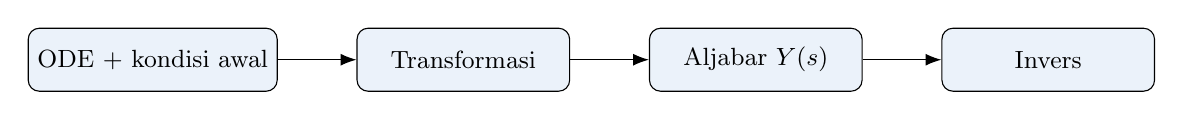
\begin{tikzpicture}[node distance=1.0cm, every node/.style={font=\small}]
\node[draw,rounded corners,fill=softBlue,minimum width=2.8cm,minimum height=0.8cm] (a) {ODE + kondisi awal};
\node[draw,rounded corners,fill=softBlue,minimum width=2.7cm,minimum height=0.8cm,right=of a] (b) {Transformasi};
\node[draw,rounded corners,fill=softBlue,minimum width=2.7cm,minimum height=0.8cm,right=of b] (c) {Aljabar $Y(s)$};
\node[draw,rounded corners,fill=softBlue,minimum width=2.7cm,minimum height=0.8cm,right=of c] (d) {Invers};
\draw[-{Latex[length=2mm]}] (a) -- (b);
\draw[-{Latex[length=2mm]}] (b) -- (c);
\draw[-{Latex[length=2mm]}] (c) -- (d);
\end{tikzpicture}
\end{center}
\[
\text{ODE } y(t) \quad \longrightarrow \quad \text{persamaan } Y(s) \quad \longrightarrow \quad \text{solusi } y(t).
\]
\end{frame}

\begin{frame}{Mini Contoh: $y'-y=0$}
\begin{exampleblock}{Soal}
\[
 y'-y=0, \qquad y(0)=3.
\]
\end{exampleblock}
Transformasi:
\[
\lap{y'}-\lap{y}=0
\]
\[
(sY-3)-Y=0.
\]
\[
(s-1)Y=3
\quad \Rightarrow \quad
Y=\frac{3}{s-1}.
\]
Invers:
\[
\boxed{y(t)=3e^t.}
\]
\end{frame}

\begin{frame}{Bandingkan dengan Separabel}
Soal yang sama:
\[
 y'=y, \qquad y(0)=3.
\]
Dengan separabel:
\[
\frac{1}{y}\dd y=\dd t
\Rightarrow \ln|y|=t+C
\Rightarrow y=Ce^t.
\]
Dengan Laplace:
\[
(sY-3)-Y=0 \Rightarrow Y=\frac{3}{s-1}\Rightarrow y=3e^t.
\]
\begin{center}
Untuk soal mudah, separabel lebih cepat. Laplace menjadi kuat ketika struktur ODE dan kondisi awal lebih kompleks.
\end{center}
\end{frame}

\begin{frame}{Contoh yang Tidak Separabel Sederhana}
\begin{block}{Contoh linear orde satu}
\[
 y'+2y=e^{-t}, \qquad y(0)=0.
\]
\end{block}
Ini tidak langsung menjadi
\[
 A(y)\dd y=B(t)\dd t.
\]
Tetapi dengan Laplace:
\[
(sY-0)+2Y=\frac{1}{s+1}.
\]
\[
Y=\frac{1}{(s+1)(s+2)}.
\]

dan nanti dapat dicari inversnya dengan tabel atau pecahan parsial.
\end{frame}

\begin{frame}{Latihan Konsep: Pilih Alat}
Untuk setiap ODE, tentukan apakah lebih cocok: integrasi langsung, separabel, operator, atau mulai diarahkan ke Laplace.
\begin{enumerate}
  \item $x''=g$.
  \item $y'=4y$.
  \item $v'=g-kv$.
  \item $y''+5y'+6y=0$.
  \item $y''+4y'+4y=t^2e^{-2t}$, dengan $y(0)=0$, $y'(0)=0$.
  \item $\theta''+\sin\theta=0$.
\end{enumerate}
\end{frame}

\begin{frame}{Kesalahan yang Sering Terjadi}
\begin{enumerate}
  \item Melupakan konstanta integrasi.
  \item Menghapus nilai mutlak pada $\ln|y|$ tanpa alasan.
  \item Tidak menggunakan kondisi awal.
  \item Menganggap semua ODE bisa dipisahkan.
  \item Menganggap operator $D$ bisa selalu diperlakukan seperti variabel biasa.
  \item Salah membaca homogen: ruas kanan nol atau homogen dalam arti lain.
\end{enumerate}
\end{frame}

\begin{frame}{Rangkuman Pertemuan}
\begin{block}{Hari ini}
\begin{enumerate}
  \item ODE adalah model perubahan.
  \item Separabel selesai dengan memisahkan variabel dan mengintegralkan.
  \item Eksponen dan logaritma muncul secara alami dari integrasi $dy/y$.
  \item Operator $D$ membantu ODE linear koefisien konstan.
  \item Tidak semua ODE cocok dengan separabel atau operator sederhana.
  \item Transformasi Laplace mengubah fungsi $f(t)$ menjadi $F(s)$ dan mengubah turunan menjadi bentuk aljabar.
\end{enumerate}
\end{block}
\end{frame}

\begin{frame}{Latihan Penutup}
Kerjakan sebagai latihan singkat.
\begin{enumerate}
  \item Selesaikan $\dfrac{dy}{dt}=-3y$, $y(0)=12$.
  \item Selesaikan $\dfrac{dv}{dt}=9.8-0.4v$, $v(0)=0$.
  \item Gunakan operator untuk menyelesaikan $y''+3y'+2y=0$.
  \item Hitung $\lap{1}$ langsung dari definisi.
  \item Gunakan tabel untuk menentukan $\lap{e^{-2t}}$, $\lap{\sin 3t}$, dan $\lap{\cos 3t}$.
\end{enumerate}
\end{frame}

\begin{frame}{Referensi}
\begin{enumerate}
  \item Mary L. Boas, \textit{Mathematical Methods in the Physical Sciences}, Chapter 8: Ordinary Differential Equations.
  \item Modul Matematika 3 Teknik Kelautan: Pekan 1-4.
  \item PR Matematika 3: Tugas 01 dan Tugas 02.
\end{enumerate}
\end{frame}

\end{document}
